\RequirePackage{cmap}
\documentclass[12pt, a4paper]{article}
\usepackage{graphicx}         % fuer das Einbinden von Grafiken
%\usepackage[ngerman]{babel}   % weglassen, wenn in Englisch
\usepackage[utf8]{inputenc}
\usepackage[T1]{fontenc} % für Silbentrennung bei Umlauten 
\usepackage{color}
\usepackage{verbatim} % für Comment Blöcke
\usepackage{siunitx}
\usepackage{amsmath}
\usepackage{amssymb}
%% \usepackage{subfigure}
\usepackage{setspace}    % um Zeilenabstände zu setzen
\onehalfspacing	% setzt Zeilenabstand auf 1,5
\setlength{\parindent}{0mm} % Einrücken der ersten Zeile eines Absatzes
\usepackage{geometry}
\geometry{lmargin=20mm,rmargin=50mm,tmargin=25mm,bmargin=25mm}
\setlength{\emergencystretch}{1em} % Verhindert overfull hbox
\usepackage[bottom]{footmisc} % Damit Fußnoten bei nicht vollen Seiten unten sind


\begin{document}

\section{Introduction}
\subsection{A Brain Atlas}
An Atlas is a relation of a Voxel, a 3D-Pixel, and a label.
Each Voxel can be represented by its position in a three dimensional coordinate system. The coordinate system used in brain imaging is gridded. So each voxels coordinates can be represented by three natural numbers. 

You can think of the labels assigned to voxels in an atlas as the name of an anatomical region, e.g. ``Visual Cortex''.
For the sake of simplicity we will assume that all labels are natural numbers instead of character strings. The relation between label numbers and the anatomical names can be handled outside of the atlas. 
Overall the atlas $A$ is relation from the three dimensional coordinate space to the one dimensional label space.
\begin{equation}
 A \colon \mathbb{N}^{3}  \rightarrow \mathbb{N}
\end{equation}
We call a set of coordinates with the same label a region.
E.g. all coordinates that relate to label $i$ form region $i$, $R_i$.
\begin{equation}
 R_i = \{ x \in \mathbb{N}^3 \mid A\left(x\right) = i \}
\end{equation}
By convention the label $0$ relates to the voxels that do not belong to the brain, e.g. the skull and surrounding space, or parts of the brain that are not of interest, e.g. the ventricles or white matter.
So the regions of interest are
\begin{equation}
 R_n, n \in \mathbb{N}_{>0}
\end{equation}

We call the cardinality of a region $|R_n|$ its size.
Given the external relation between the voxel grid and physical space we can calculate the volume of a region. 
This external relation is defined by the ``Space'' of the image.
The atlases used in this work are in MNI152 space. Each image voxel represents a physical space of $1\times1\times1 ~\text{mm}^3$.
So a region of size $1000$ has a volume of $1~$mL.

We define as the diameter of region $R_i$ the maximum distance of two members of $R_i$
\begin{equation}
 diam(R_i) = \max_{x,y \in R_i} |x-y|
\end{equation}



\subsection{The Harvard-Oxford cortical and subcortical atlases}
The Harvard-Oxford cortical and subcortical atlases are two atlases labeling 48 cortical and 21 subcortical anatomical regions.

The regions in the Harvard-Oxford cortical atlas have a volume of $ ( 22.0  \pm 22.2 )  ~\text{ml}$.
Notably two anatomical structures in the left and right hemisphere that are each others mirrored counterpart are labeled the same and thus form the same region, even if the two structures do not ``touch''.

The Harvard-Oxford cortical atlas labels 21 regions with a volume of $ ( 78  \pm 157 )  ~\text{ml}$. These include large ``Cortex'' regions which are labeled in more detail in the cortical atlas and white matter and ventricles, which are of no interest for our atlas.

\section{Combined subparcellated atlas}
\subsection{Motivation}
From the Harvard-Oxford cortical and subcortical atlases we want to derive an atlas with these properties:
\begin{enumerate}
 \item Each region is a subset of a region in the Harvard-Oxford atlases
 \item Cortical regions are either in the left or right hemisphere, not both
 \item The mean volume of the regions is 2ml
 \item The variance of region volumes is minimized
 \item The regions diameter is minimized.
\end{enumerate}

Property 1 allows us to assign the same names of anatomical structures to regions, as the Harvard-Oxford atlases do. 
Property 2 satisfies our physical understanding that structures that are spatially separated are not identical.
Properties 3 and 4 will allow us the assumption, that the volume of all regions is the same, simplifying diffusion-advection equations.
Property 5 will allow us the assumption, that diffusion influenced concentrations are homogeneous within the region.


\subsection{Combining}
Some voxels have a label in both Harvard-Oxford atlases. For example the region Cortex in the subcortical atlas, which is is labeled in more detail in the cortical atlas.

We therefore remove these regions from the atlas with the less detailed labeling for the respective anatomical structures. From the cortical atlas we remove
\begin{itemize}
 \item Parahippocampal Gyrus, anterior division
 \item Parahippocampal Gyrus, posterior division
\end{itemize}
From the subcortical atlas we remove
\begin{itemize}
 \item Left Cerebral Cortex 
 \item Right Cerebral Cortex 
\end{itemize}
Also we remove from the subcortical atlas
\begin{itemize}
 \item Left Cerebral White Matter
 \item Right Cerebral White Matter
 \item Left Lateral Ventricle
 \item Right Lateral Ventricle
\end{itemize}
because these anatomical structures are not relevant for tau pathologies.

After this step 1.14 million voxel have a label in either of the two atlases.
Of these only four voxel have a label in both atlases. These four have been manually assigned to one of the two possible regions. 
Now both atlases can be combined into one. The label numbers are chosen such that no two region have the same label number.

Some regions $R_i$ are composed of disjointed components.
\begin{align}
C_1 \cup C_2 = R_i\\ 
C_1 \cap C_2 = \emptyset \\
 \min_{x \in C_1,y \in C_2} |x-y| > \theta
\end{align}
where $\theta$ is the minimum distance between two components of the region. For two anatomical structures in the left and right hemisphere labeled as the same region, $C_1$ and $C_2$ are of comparable size and $theta$ is large. For these cases we split the region and make each component its own region.
Some regions have disjointed components composed of just a few voxel, and small $theta$. Those regions are kept as is.

After this separation the ``Frontal Pole'' is the only region that does not satisfy property 2 from Section 2.1, being in the left or right hemisphere exclusively. The region was split manually based on voxel coordinates.

\subsection{Subparcellation}
We sort the regions by size. Starting with the largest we will parcellate the regions into smaller regions. We want regions of 2mL Volume. We devide the largest regions Volume by 2mL to find the number $k$ of subregions we want.
Once the largest region is split, we choose the next largest region and repeat the process until the average region volume is 2mL, satisfying Property 3 from Section 2.1.

To parcellate region $R_i$ into $k$ subregions we randomly choose $k$ distinct seeds $x_j \in R_i$. This gives us $k$ components $C_j = \{ x_j \}$, $C_j \subset R_i$.

Sort the $C_j$ by size in decreasing order (in the beginning all have size one, this will change).
Add to the smallest $C_j$ all elements from $R_i$ that are within some distance $d$.
\begin{equation}
 C'_j = \{ x \in R_i \mid \exists y \in C_j : |x-y| \leq d \}
\end{equation}
Usually $C'_j$ is larger than $C_j$. Elements of $R_i$ that were formally in none of the components may now be in $C'_j$. Other components of $R_i$ may have been decreased in this step. We conserve 
\begin{equation}
 \bigcap_{C_i \neq C_j} = \emptyset
\end{equation}
to satisfy Property 1 from Section 2.1.
Remember that $C_j$ was the smallest component of $R_i$. We now sort the $C_j$ by size again and repeat the process with the new smallest component until all elements of $R_i$ are element of of of the components. That is
\begin{equation}
 \bigcup_{C_j} = R_i
\end{equation}

We now found a parcellation derived from the $k$ randomly chosen seeds.
We calculate the variance in volume of the components and the largest diameter of the components. If the diameter is above a certain threshold this parcellation is discarded to satisfy Property 5 from Section 2.1.
The process is repeated over and over with different randomly chosen seeds. 
The parcellation with the smallest variance in volume is chosen to satisfy Property 4 in Section 2.1.

\newpage
\section{Result}
The code for finding a parcellation that minimizes the standard deviation (SD) in region volume and minimizes the region diameters run for 24 hours on a latptop with i5 processor. The best parcellation for each original region was chosen to create the atlas with the following properties.
\begin{center}
\begin{tabular}{r|r}
Number Regions& 571 \\
\hline \hline
Mean Volume & 2.00 mL \\
\hline 
SD Volume& 0.21 mL \\
\hline
Max Volume & 2.71 mL\\
\hline 
Min Volume & 0.67 mL\\
\hline \hline
Mean Region Diameter & 27.2 mm \\
\hline 
SD Region Diameter & 8.5 mm\\
\hline
Max Region Diameter & 41.9 mm\\
\hline
Min Region Diameter & 18.2 mm
\end{tabular}
\end{center}

\begin{figure}
\centering
\begin{minipage}{.5\textwidth}
  \centering
  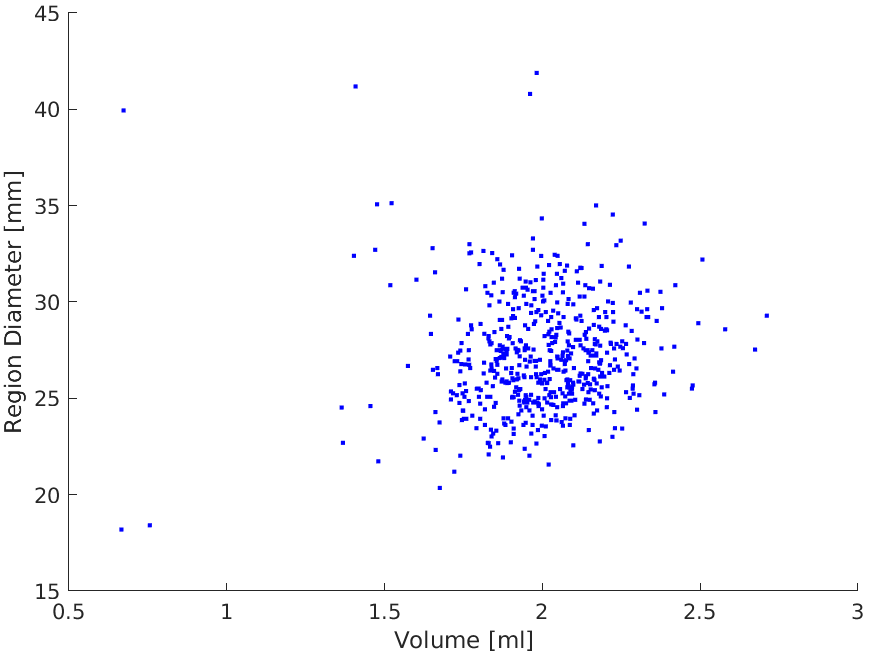
\includegraphics[width=\linewidth]{2018-09-17_diameter_volume.png}
  \caption{Distribution of region diameter and volume}
  %\label{fig:volumes}
\end{minipage}%
\begin{minipage}{.5\textwidth}
  \centering
  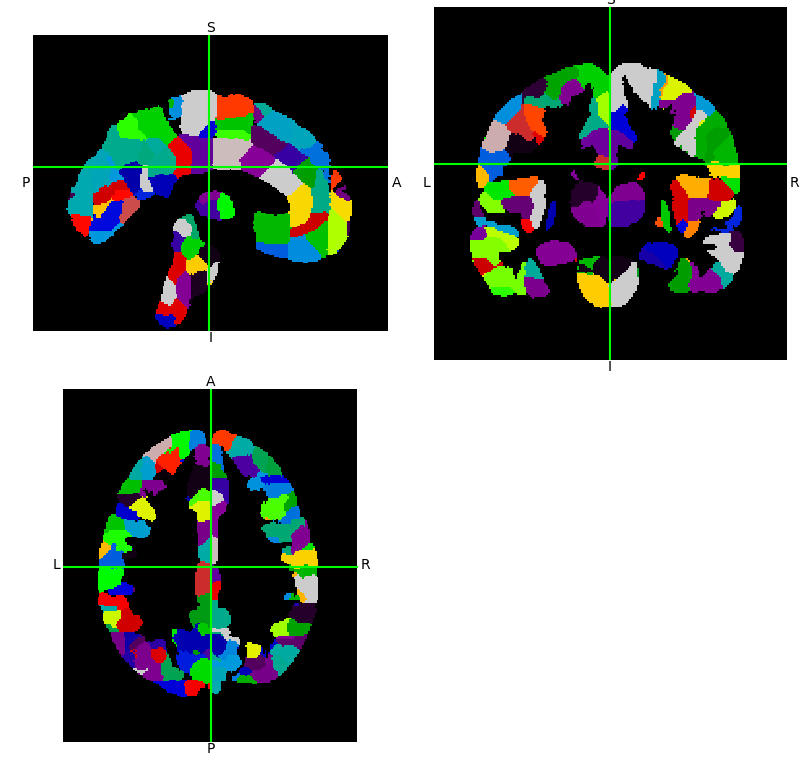
\includegraphics[width=\linewidth]{combined_atlas_new_labels_2018_09_17}
  \caption{Resulting Atlas}

\end{minipage}
\end{figure}

The distribution of region diameters and volume is shown in Fig. 1.
The Atlas itself in Fig. 2.

\end{document}
